% begin module transformations-shifts-example
\begin{frame}
\begin{example}[Example 2, p. 39]
Draw a graph of the function $f(x) = x^2 + 6x + 10$.
\begin{columns}[c]
\column{.5\textwidth}
\ \only<handout:0| -6>{%
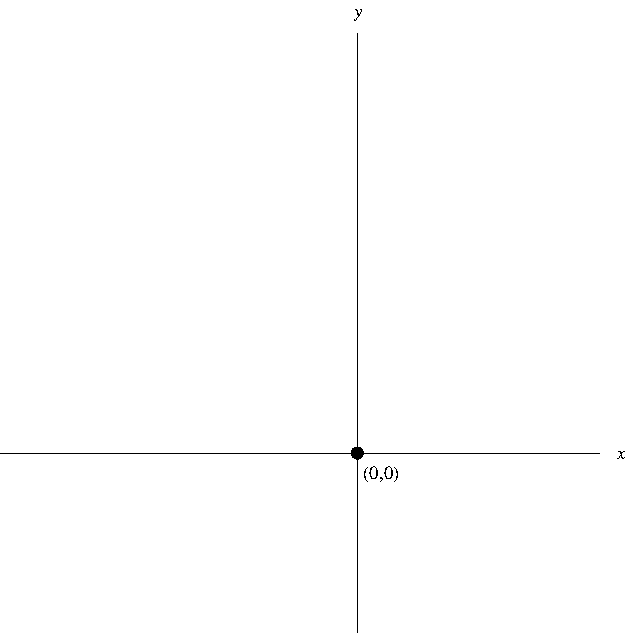
\includegraphics[height=5cm]{precalculus/pictures/01-03-parabolaa.pdf}%
}%
\only<handout:0| 7>{%
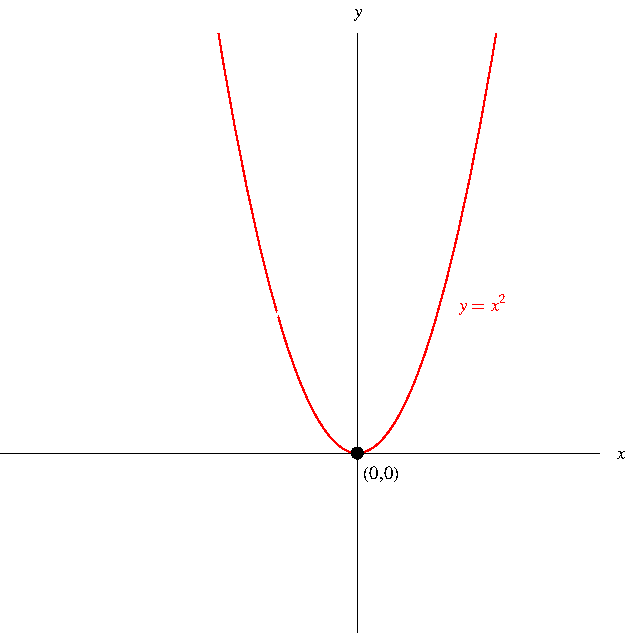
\includegraphics[height=5cm]{precalculus/pictures/01-03-parabolab.pdf}%
}%
\only<8->{%
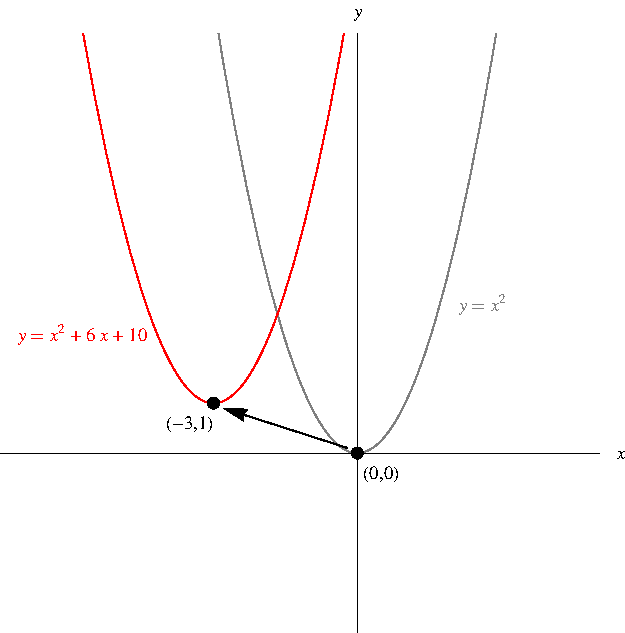
\includegraphics[height=5cm]{precalculus/pictures/01-03-parabolac.pdf}%
}%
\column{.5\textwidth}
\uncover<2->{
Complete the square:
}
\begin{eqnarray*}
\uncover<3->{f(x)} & \uncover<3->{ = } & \uncover<3->{x^2 + 6x + 10} \\
& \uncover<4->{ = } & \uncover<4->{(x^2 + 6x \uncover<5->{\alert<handout:0| 5>{+ 9}}) + 10 \uncover<5->{\alert<handout:0| 5>{- 9}}} \\
 & \uncover<6->{ = } & \uncover<6->{(x + 3)^2 + 1} \\
\end{eqnarray*}
\end{columns}
\end{example}
\end{frame}
% end module transformations-shifts-example
